\documentclass[aspectratio=169,10pt]{beamer}

% Same look as the seminar presentation.
\usetheme{metropolis}
\metroset{block=fill, numbering=fraction}

\usepackage{tikz}
\usetikzlibrary{arrows.meta,positioning}
\usepackage{array,booktabs}
\usepackage{xcolor}

\definecolor{giublue}{RGB}{30,58,138}
\definecolor{giuaccent}{RGB}{13,148,136}
\setbeamercolor{frametitle}{bg=giublue}
\setbeamercolor{progress bar}{fg=giuaccent}
\setbeamercolor{alerted text}{fg=giuaccent}
\setbeamerfont{title}{size=\large}
\setbeamerfont{subtitle}{size=\small}

\title{Learning Each Person's Comfort Zone}
\subtitle{Personalised greeting with reinforcement learning, on the Yanshee robot}
\author{Nour Gaser \and Eman Saleh}
\institute{German International University}
\date{Seminar project demo}

\begin{document}

\maketitle

% ------------------------------------------------------------------
\begin{frame}{The question}
People differ in how close they want a robot to come and how loudly they want
to be greeted. A robot can learn these preferences from how people react.

\bigskip
\alert{Does it need a different behaviour for each person, or is one
well-trained behaviour enough for everyone?}

\bigskip
The papers we reviewed (Wang et al.\ 2025, Tozadore et al.\ 2018,
Gonzalez-Santocildes et al.\ 2024, Zedda et al.\ 2023) show that robots can
adapt, but rarely compare against a trained single policy.
\end{frame}

% ------------------------------------------------------------------
\begin{frame}{What the robot sees, does, and learns from}
\begin{columns}[T]
\column{0.5\textwidth}
\textbf{State} (12 situations)
\begin{itemize}
  \item distance to the person: intimate, personal, social, far
  \item its own greeting strength: low, medium, high
\end{itemize}
\textbf{Actions} (5)
\begin{itemize}
  \item step closer, step back
  \item greet more strongly, more softly
  \item hold
\end{itemize}
\column{0.5\textwidth}
\textbf{Reward}, from the person's reactions only
\begin{itemize}
  \item touch on the robot: $+1$
  \item the person leaves: $-2$, interaction ends
  \item every step: $-0.05$
\end{itemize}
\textbf{Learning}: tabular Q-learning, a $12 \times 5$ table per person.

\medskip
Three simulated people with hidden preferences: \emph{reserved} (far, quiet),
\emph{neutral} (personal distance, medium), \emph{sociable} (close, loud).
\end{columns}
\end{frame}

% ------------------------------------------------------------------
\begin{frame}{One policy per person, or one for everyone}
\centering
\begin{tabular}{lrrr}
\toprule
 & reserved & neutral & sociable \\
\midrule
scripted greeting       & $-1.26$ & $2.03$ & $-0.75$ \\
one policy for everyone & $6.45$  & $-0.75$ & $-0.75$ \\
best single policy      & $11.81$ & $-0.75$ & $-0.75$ \\
\textbf{one policy per person} & $\mathbf{11.83}$ & $\mathbf{10.31}$ & $\mathbf{8.34}$ \\
\bottomrule
\end{tabular}

\medskip
{\small Mean reward per interaction, 8 seeds, 6000 training episodes each.}

\bigskip
\raggedright
The best single policy suits the reserved user and does worse than the scripted
greeting for the other two. Learning a separate policy per person gains $+11.06$
and $+9.09$ on those two.

\medskip
Pre-training on other people did not help a new person learn faster. Here the
preference is the whole task, so there is nothing general to transfer.
\end{frame}

% ------------------------------------------------------------------
\begin{frame}{Moving the same code to the Yanshee}
\begin{columns}[T]
\column{0.42\textwidth}
\centering
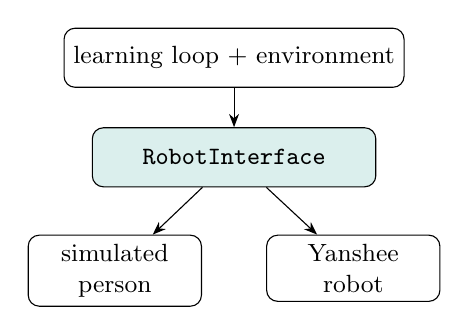
\begin{tikzpicture}[
  box/.style={draw, rounded corners, align=center, font=\small,
              minimum width=3.6cm, minimum height=0.75cm},
  >=Stealth]
\node[box] (env) {learning loop + environment};
\node[box, below=0.5cm of env, fill=giuaccent!15] (ri) {\texttt{RobotInterface}};
\node[box, below left=0.6cm and -1.4cm of ri, minimum width=2.2cm] (mock) {simulated\\person};
\node[box, below right=0.6cm and -1.4cm of ri, minimum width=2.2cm] (yan) {Yanshee\\robot};
\draw[->] (env) -- (ri);
\draw[->] (ri) -- (mock);
\draw[->] (ri) -- (yan);
\end{tikzpicture}

\medskip
{\small The learning code is unchanged; only the robot class is new.}

\column{0.56\textwidth}
\small
\begin{tabular}{@{}ll@{}}
\toprule
interface & on Yanshee \\
\midrule
step closer / back & walk forward / backward \\
greeting strength & volume, gesture, spoken greeting \\
distance & infrared sensor \\
touch (reward) & touch sensor \\
person left & infrared sees nobody \\
\bottomrule
\end{tabular}

\medskip
Yanshee is 37\,cm tall, so the distance zones are scaled by $1/3$ onto a
table: 15, 30 and 50\,cm.

\medskip
Policies are learned in simulation (about one second each) and run on the
robot without further learning.
\end{columns}
\end{frame}

% ------------------------------------------------------------------
\begin{frame}{The live demo}
A person plays one of the simulated users, following its rules.

\begin{enumerate}
  \item \textbf{Reserved policy, reserved person.} The robot stops at a
        distance and greets quietly.
  \item \textbf{Sociable policy, sociable person.} The robot walks up close
        and greets loudly.
  \item \textbf{Sociable policy, reserved person.} The robot comes too close and
        the person leaves. This is the result in the table, in one interaction.
\end{enumerate}
\end{frame}

% ------------------------------------------------------------------
\begin{frame}{Limitations}
\begin{itemize}
  \item The users are simulated, and in the demo a person plays one. This shows
        the behaviour transfers to a robot, not how real people react.
  \item Tabular Q-learning on 12 states: easy to inspect, trains in a second,
        but too small for richer sensing.
  \item Three user types, no user study, no subjective measures.
  \item The robot is told which person it is greeting; recognising them is
        future work.
\end{itemize}

\bigskip
\centering
Code, results and documents: \texttt{github.com/nourgaser/nao-adaptive-rl}
\end{frame}

\end{document}
